
%(BEGIN_QUESTION)
% Copyright 2011, Tony R. Kuphaldt, released under the Creative Commons Attribution License (v 1.0)
% This means you may do almost anything with this work of mine, so long as you give me proper credit

Beregn nødvendig høyde på radioantennene (anta samme høyde for begge) for at første Fresnel-sone skal være fri for interferens. Anta en signalfrekvens på 900 MHz, og at de to objektene i figuren ligger nøyaktig langs siktlinjen mellom antennene:

$$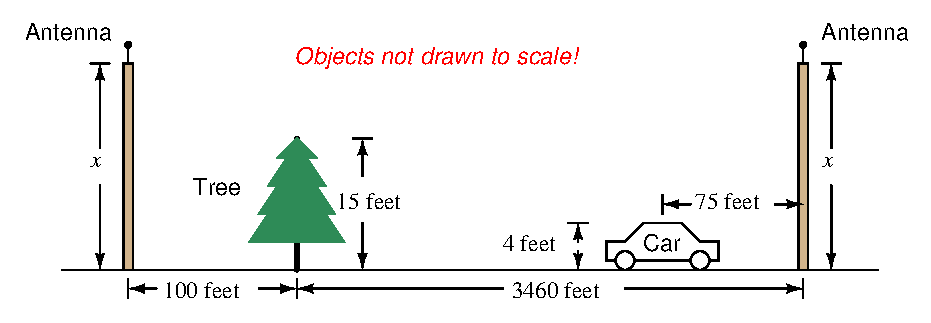
\includegraphics[width=15.5cm]{i00518x01.eps}$$

\vskip 20pt \vbox{\hrule \hbox{\strut \vrule{} {\bf Forslag til sokratisk diskusjon} \vrule} \hrule}

\begin{itemize}
\item{} Hvis du skulle designe dette antennesystemet, hvilke andre forhold ville du vurdert når det gjelder antennehøyde og objekter som kan trenge inn i Fresnel-sonen?
\item{} Anta at reguleringsbestemmelser forbyr antennemast høyere enn 20 fot. Foreslå egnede løsninger for radiolinken med denne begrensningen.
\end{itemize}

\underbar{file i00518}
%(END_QUESTION)





%(BEGIN_ANSWER)

Hvis du kom frem til en minimum antennehøyde på omtrent 26 fot, glemte du en viktig beregning av Fresnel-sonens radius. Minimum høyde for begge antenner er faktisk over 31 fot.

%(END_ANSWER)





%(BEGIN_NOTES)

Det er verdt å merke seg at alle RF-beregninger som involverer avstand (inkludert Fresnel-sone-bredde) kan utføres i britiske enheter i stedet for SI, så lenge alle størrelser bruker kompatible enheter. Det betyr lyshastighet i {\it feet} per sekund, bølgelengde i {\it feet}, osv. Lyshastigheten er nøyaktig 299792458 meter per sekund, som omregnet til feet per sekund blir:

$$\left(299792458 \hbox{ m} \over \hbox{s} \right) \left(100 \hbox{ cm} \over 1 \hbox{ m} \right) \left(1 \hbox{ in} \over 2.54 \hbox{ cm} \right)  \left(1 \hbox{ ft} \over 12 \hbox{ in} \right) = 9.8357 \times 10^{8} \hbox{ ft/s}$$

Med dette kan vi beregne signallengden ved 900 MHz:

$$v = \lambda f$$

$$\lambda = {v \over f} = {9.8357 \times 10^{8} \hbox{ ft/s} \over 900 \times 10^6 \hbox{ Hz}} = 1.0929 \hbox{ ft}$$

\vskip 10pt

Radiusen til en Fresnel-sone er gitt av følgende formel:

$$r = \sqrt{{n \lambda d_1 d_2} \over D}$$

\vskip 10pt

Løst for $r$ i en avstand på 100 fot fra én antenne (dvs. $d_1$ = 100 ft ; $d_2$ = 3460 ft ; $D$ = 3560 ft):

$$r = \sqrt{{(1) (1.0929) (100) (3460)} \over 3560} = 10.306 \hbox{ ft}$$

Dermed er radiusen i første Fresnel-sone ved 100 fot fra antennen 10.306 fot. For å klarere treet på 15 fot må antennen være minst 25.306 fot høy.

\vskip 10pt

Ser vi på hinder nummer to (bilen), må den allerede være utenfor første Fresnel-sone dersom sonen klarerer treet og begge antennene står i samme høyde, siden treet er både høyere og lenger unna sin antenne enn bilen. Likevel, for øvelse:

$$r = \sqrt{{(1) (1.0929) (75) (3485)} \over 3560} = 8.958 \hbox{ ft}$$

På dette grunnlaget må antennen være minst 12.958 fot høy for å klarere bilen på 4 fot.

\vskip 10pt

Maksimal bredde i første Fresnel-sone finnes ved å sette $d_1$ og $d_2$ i midtpunktet av totalavstanden 3560 fot ($d_1 = d_2$ = 1780 ft):

$$r = \sqrt{{(1) (1.0929) (1780) (1780)} \over 3560} = 31.187 \hbox{ ft}$$

Maksimal Fresnel-radius (i midten) = 31.187 fot. Dermed er interferens fra bakken den mest sannsynlige formen for interferens i første Fresnel-sone, og dette krever antenner på minst 32 fot (avrundet opp til nærmeste hele fot). Setter vi begge antennene høyt nok til at Fresnel-sonen klarerer bakken i midtspennet, klarerer vi lett både treet og bilen.











\vfil \eject

\noindent
{\bf Oppsummeringsquiz:}

Anta at en radiolink oppgraderes fra 900 MHz-transceivere til 2.4 GHz-transceivere. Hvilken innvirkning vil denne endringen i driftsfrekvens ha på radiusen i Fresnel-sonen (i et vilkårlig punkt)?

\begin{itemize}
\item{} Den nye Fresnel-sonen blir større: 163\% av størrelsen til den gamle Fresnel-sonen
\vskip 5pt 
\item{} Den nye Fresnel-sonen blir større: 711\% av størrelsen til den gamle Fresnel-sonen 
\vskip 5pt 
\item{} Den nye Fresnel-sonen blir mindre: 61.2\% av størrelsen til den gamle Fresnel-sonen
\vskip 5pt 
\item{} Den nye Fresnel-sonen blir mindre: 37.5\% av størrelsen til den gamle Fresnel-sonen 
\vskip 5pt 
\item{} Den nye Fresnel-sonen blir større: 267\% av størrelsen til den gamle Fresnel-sonen 
\vskip 5pt 
\item{} Den nye Fresnel-sonen blir mindre: 14.1\% av størrelsen til den gamle Fresnel-sonen 
\end{itemize}


%INDEX% Electronics review, Fresnel zones for radio links

%(END_NOTES)
